\documentclass[../../main.tex]{subfiles}

\begin{document}
    
    \section{Steganalysis}
    Steganalysis is the branch of study dedicated at analysing the methods and
    the vectors used to transmit an hidden message in order to retrieve such
    message whenever it is present.
    Unlike cryptanalysis where the message may even be apparent but encrypted,
    in steganalysis the study of the message starts from a suspect.
    \subsection{Methods}
    Hereinafter we will present the methods used in steganalysis in
    order to obtain the secret message. The following image illustrates all of them. Here we simply want to introduce them in a rigorous way, but they will be treated 
    in the specific cases when dealing with the cover types.

    \begin{figure}[h]
        \centering
        \caption{Steganalysis techniques}
        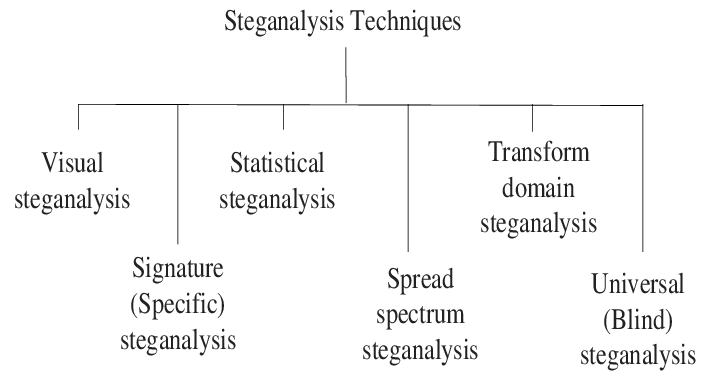
\includegraphics[scale=0.4]{classification_steganalysis.png}
    \end{figure}


    \subsubsection{Statistical}
    Statistical steganalysis consists in using tools borrowed by Statistics in order to spot anaomalies in the cover message.
    These anomalies can be usually detected by searching in the data for patterns or by simply analysing some alteration of the modelled
    probability distribution of the data in the message. Often Neural Networks are involved in this type of steganalysis.

    \subsubsection{Visual}
    This is a very rudimental yet effective way of determining if a message was modified or not. This technique relies on the human eye and ita ability
    to spot anomalies in the format of a message which may pave the way for suspects.
    
    \subsubsection{Spread Spectrum}
    This is a technique borrowed by signal analysis which consists in treating the data on which we want to perform the analysis as a signal.
    Following this reasoning it is almost immediate to see that the stego message embedded into our data is nothing but noise in our signal. Finally the steganalysis
    is performed in this case just like any other type of signal analysis.

    \subsubsection{Signature}
    Signature is deeply correlated to the field of Watermarking. In many cases the data on which it was performed the steganography could have been signed.
    The insertion of the stego message inside the signed data may thus lead to the alteration in the digital dignature, making the message visible 
    to the receiver.
    
    \subsubsection{Transform Domain}
    Even in this case the goal is to start from considering the data we are analysing as a signal. Then we try to transport this signal from a domain into another 
    so that to make it invisible to the end user.
    
    \subsubsection{Universal}
    This is a type of analysis performed in a sort of bloind mode. In this case we don't care aboutt he medium through which the message was sent but we perform a series of 
    operations(reading LSB for example) which have little to nothing to do with the message itself.

    \subsection{Cover types}
    In the following sections, we will treat several \emph{cover} in which
    steganography can be applied to hide data.
    In particular we will focus on some of the most common methods and how is
    possible to do a steganalysis process in order to detect and in some cases
    even retrieve the embedded information.
    Notice that different cover types requires completely different approaches
    due to intrinsic factors such as size, presence of redudant data,
    perceptibility of modification by a human or formats in which the bits of
    the cover are stored.


    \subsection{Images}
    Images are likely to be chosen to hide secret messages due to the low
    sensibility of the \emph{human visual system} (HVS) to some particular
    attributes such as small changes in luminance or brightness or contrast near
    figures edges.
    There are several methods to apply steganography to an image, in the
    following sections we will treat some of the most common hiding techniques
    and some of the steganalysis methods to attack them.


    \subsubsection{Stego-key search and encryption}
    When in the following sections we will mention modification applied to
    \emph{LSB} of some data characterizing the images, it's crucial to mention
    that not always all LSB are modified nor are modified in subsuqeunt blocks.
    More complex steganographic techniques imply the use of some pseudo-random
    walk followed when deciding which data to modify, generated by some
    \emph{stego-key} (usually stego-key will be mapped in a set of possible
    seeds by a hash map) \cite{stego-key}.

    It's also possible to apply an \emph{encryption} algorithm before embedding
    the message in order to make steganalysis harder, since the attacker cannot
    find any recognizable bit sequence, when searching for the message.

    The use of such systems makes the steganalysis process much harder since it
    becames unfeasible the use of a brute force approach: the complexity would
    be proportional to the cardinality of the set of possible seeds time the
    one of the set of possible encryptions.

    Moreover, even if the LSB are modified in blocks and no encryption is
    applied, the steganalysis methods are useful to comprehend (without need to
    find recognizable bit sequences) if the images contains secret messages in
    a systematic way.


    \subsubsection{LSB embedding method}
    LSB embedding method is arguably the most popular steganographic method, due
    to its simplicity, high imperceptibility and high capacity.
    In this method, the image is decomposed into \emph{bits plane} (8 bits per
    pixel for grayscale and 24 for color images, one for each color channel)
    and the \emph{least significant bit} (LSB) is substituted with the message
    to be hidden.
    Note that even if the message is encrypyted, due to its simplicity, this
    method is easily detectable with a statistical steganalysis attack
    \cite{techniques-data-hiding}.
    

    \subsubsection{Difference Image Histogram method}
    The \emph{Difference Image Histogram method} is derived by the easier idea
    of analysing the \emph{histogram distribution} of a natural image and its
    stegoimage. Anyway, when we are steganalysing an image, we \emph{do not}
    have the natural image, so what we could do is comparing the histogram
    distribution of the suspect image with a set of natural images, but the
    problem is that the variation between two different images is \emph{bigger}
    than the distribution variation between a natural image and its stegoimage.
    \cite{methodology-steganalysis-images}

    The proposed way to proceed is the following
    \cite{new-detection-lsb-steganography}, starting from the test image (that
    we will call $h$, considering $h$ a grayscale image or a color image under
    some assumptions) we generate:
    \begin{enumerate}
        \item an image $f$ given by $h$ with flipped LSB
        \item an image $g$ given by $h$ zeroing the LSB
        \item images $D_h$, $D_f$, $D_g$, created by the respective image of
              each one with the following formula:

              \[ D(i,j) = I(i+1,j) - I(i,j) \]

              where $I$ is the image denoted by the subscript and the couple
              $(i,j)$ a unique pixel of the image
    \end{enumerate}

    At this point, we can analyse the histograms of the three generated images
    $D_h$, $D_f$, $D_g$:

    \[
        H = \{h_i | i = -255,\ ...,\ +255\},\ 
        F = \{f_i | i = -255,\ ...,\ +255\},\ 
        G = \{g_i | i = -255,\ ...,\ +255\}
    \]

    \begin{figure}[h]
        \centering
        \caption{Transition values from $G$ to $H$ and $F$}
        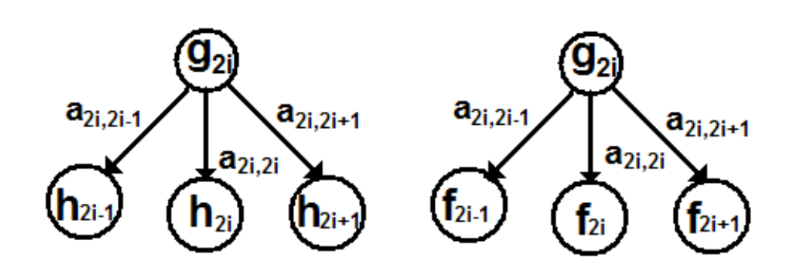
\includegraphics[scale=0.4]{difference_histogram_mtd.png}
    \end{figure}

    then, we define the following values:

    \[ \alpha_i = \frac{a_{2i+2,2i+1}}{a_{2i,2i+1}} \]
    \[ \beta_i = \frac{a_{2i+2,2i+3}}{a_{2i,2i-1}} \]
    \[ \gamma_i = \frac{g_{2i}}{g_{2i+2}} \]

    As found out by X. Ping and T. Zhang in
    \cite{new-detection-lsb-steganography}:

    \begin{itemize}
        \item if $\alpha_i \approx 1, \forall i \in \{-255, -254, ..., 255\}$
              then the image contains some hidden message;
        \item otherwise, for natural images, $\alpha_i \approx \gamma_i$ is
              satisfied.
    \end{itemize}
    
    \subsubsection{Closest Color Pair method}
    Another method used to detect hidden messages on the LSB plane is the
    \emph{Closest Color Pair method}.

    Whhen an image has a steganographed message in te LSB plane, the number of
    close colors increases \cite{detecting-lsb-steganography}. Given two pair of
    colors $C_1=[R_1,G_1,B_1],\ C_2=[R_2,G_2,B_2]$, the condition of them being
    close is:

    \[ (R_1-R_2)^2+(G_1-G_2)^2+(B_1-B_2)^2 \leq 3 \]

    We apply a LSB embedding steganography algorithm on the image and we compute
    the number of close color pairs in both images.

    Now, we define:

    \begin{itemize}
        \item $P$ as the number of close color pairs; $P'$ as the number of
              close color pairs of the stegoimage;
        \item $U$ as the number of color pairs; $U'$ as the number of color
              pairs of the stegoimage
    \end{itemize}

    Then, we compute:

    \[ R = \frac{P}{\binom{U}{2}},\ R' = \frac{P'}{\binom{U'}{2}} \]

    We know that if

    \[ \frac{R}{R'} \geq Th,\ Th = 1.1 \]

    \noindent then the image is a natural image, otherwise it contains an hidden
    message. All the proofs are in \cite{detecting-lsb-steganography}.

    \subsubsection{JPEG steganalysis}
    JPEG images are one of the most used format on Internet web sites, due to
    their high compression rate, while maintaining a good quality.
    \paragraph{DCT Domain embedding methods} modify the compression coefficients
    in order to hide data inside the image.
    The JPEG format uses a \emph{discrete cosine transform} (DCT) to transform
    every 8x8-pixel block into 64 DCT coefficients, that are used to calculate
    the pixels when the image is displayed.
    The simplest and most used DCT Domain embedding method substitute the
    \emph{LSB} of the coefficients with the secret message: since the
    modification is done in the frequency domain, there is no human perceivable
    change in the image.
    However, this modifications can be detect by analyzing the DCT coefficients
    which change significantly with respect to a natural image.
    \paragraph{Chi-square test} is a statistical steganalysis test, which aims
    at determining whether an image shows distorsion from embedding hidden data.
    \begin{enumerate}
        \item Let $n_i$ be the frequency of the DCT coefficient $i$ in the
            image, we assume that an image with hidden data has similar
            frequency for adjacent coefficients so we compute the arithmetic
            mean $y_{i}^{*} = \frac{n_{2i}+n_{2i+1}}{2}$ to derive the expected
            distribution
        \item The expected distribution is compared with the observed one
            $y_i = n_{2i}$
        \item The chi-square distribution for the difference between the
            expected and the observed DCT coefficients is calculated as follows:
            $$ \chi^2 = \sum_{i=1}^{\ni+1}
            \frac{\left( y_i-y_{i}^{*}\right)}{y_{i}^{*}}$$
            where $\ni$ are the degrees of freedom, which are one less than the
            categories in the DCT coefficients histogram
        \item The probability that there is an embedded message can be computed
            as the complement of the \emph{cumulative distribution function} of
            the chi-square distribution
    \end{enumerate}
    Note that, as presented in the stego-key section, different algorithms
    modify the coefficients not sequentially or following different orders, so
    the steganalysis process is usually performed by calculating the probability
    of the presence of an embedded message considering different portions of the
    image at the same time.
    


    \subsection{Audio}
    Steganography in audio is more challenging with respect to images, because
    the \emph{human auditory system} (HAS) operates over a wide dynamic range,
    while maintaining a high sensitivity to perturbations and noises.
    Howerer, there are still some ``holes'' where data can be hidden.
    The HAS has a quite small differential range, so loud sounds mask out quiet
    sounds, moreover it is unable to perceive absolute sound phase, but only
    relative one.

    Another important factor to consider when dealing with sound are the
    transmissions enviroments.
    Audio signals can be transmitted through a digital channel (eventually being
    resampled), through an analog channel or ``over the air'' played by a
    speaker and received by a microphone.
    Depending on the transmission channel there could be huge modification that
    can make the steganalysis process impossible, but also that can compromise
    irreparably the hidden message, damaging also the steganographer
    \cite{techniques-data-hiding}.

    Due to the several issues presented above, steganalysis in audio signals is
    more complex with respect to other cover types.
    In the following sections we will cover some of the possible ways in which
    steganography and steganalysis is applied in audio signals.

    \subsubsection{Non-compressed and compressed methods}
    We can distinguish two different types of audio steganography: steganography
    on \emph{non-compressed} audio files and on \emph{compressed} ones.
    The first ones aims at exploiting the vulnerabilities of the \emph{HAS}
    presented above, whereas the second ones perform minor modifications to
    embedd data based on the way in which the compression is perfomed
    \cite{review-audio-steganalysis}.

    \subsubsection{Phase coding}
    The phase encoding method works by modifying the \emph{absolute phase} of
    audio signals to convey information, while maintaining the \emph{relative
    phase} in order to not compromise imperceptibility.

    \paragraph{Encoding procedure} can be performed as follows
    \cite{techniques-data-hiding}:
    \begin{enumerate}
        \item The sound is broken into a series of N short segments
        \item A \emph{discrete Fourier transform} (DFT) is applied to every
            segment constructing two matrices: one for the \emph{phase}
            $\phi_n(\omega)$ and the other for the \emph{magnitude}
            $A_n(\omega)$ of every segment
        \item The phase difference between each adjacent segment is stored
        \item The binary set of data which has to be hidden is represented as
            $\frac{\pi}{2}$ or $-\frac{\pi}{2}$ respectively 0 or 1
        \item The phase matrix is recomputed embedding the message by modifying
            the phase difference between adjacent segments with the encoding
            presented at the previous point
        \item Finally the \emph{modified phase matrix} and the original
            magnitude matrix are used to reconstruct the sound signal b
            applying the inverse DFT
    \end{enumerate}

    \paragraph{Steganalysis techniques} for phase coding system follows a
    procedure similar to the encoding ones, since is based on a statistical
    analysis of \emph{phase discontinuites}, but which requires the use of a
    classification algorithm in order to distinguish between natural and
    modified signals.
    
    As proposed in \cite{steganalysis-phase-coding}, the steganalysis can be
    perfomed as follows:
    \begin{enumerate}
        \item The signal is divided into segments to which is applied a
            \emph{fast Fourier transform} (FFT) in order to extract the phase
            difference between adjacent segments
        \item The phase difference is monitored calculating statistical features
            of the sample
        \item \emph{SVM classifier} (support-vector machines) is used to
            detect if the signal has been modified or not
    \end{enumerate}
    A SVM classifier, after a proper training, is able to clearly distinguish
    between elements by mapping them into two different classes by means of
    linear regression and statistical calculus.
    This method is applied varying the length of segements to which the FFT is
    applied.


    \subsubsection{Echo embedding methods}
    The echo embedding methhods hide data introduzing or varying an \emph{eco}.
    \begin{figure}[h]
        \centering
        \caption{Echo kernels and parameters}
        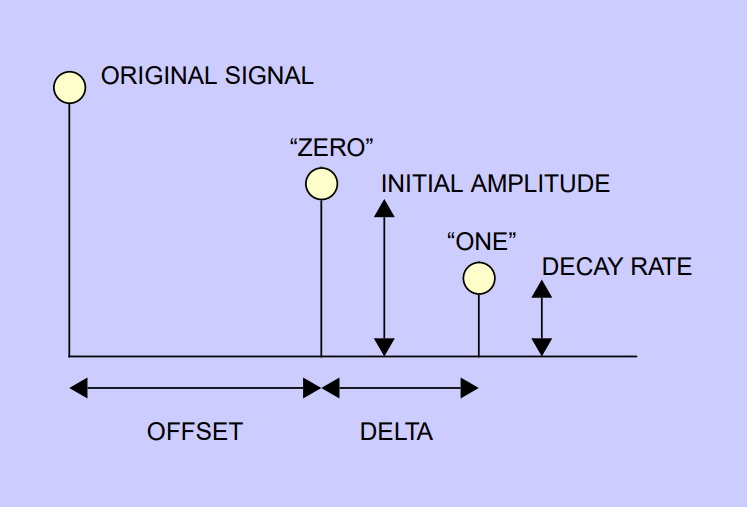
\includegraphics[scale=0.6]{audio_echo.png}
    \end{figure}
    Data are hidden by varying \emph{initial amplitude}, \emph{decay rate} and
    \emph{offset}.
    \paragraph{Encoding} is performed by dividing the signal into smaller
    portions and the echoing each portion as an independent signals by an audio
    mixing process.
    The coder use two different delay times to represent a binary zero(offset)
    and a binary one(offset+delta), both below audible threshold, considering
    the initial amplitude and that the decay rate follows and exponential
    behaviour.
    The final signal is formed by recombining all independent encoded signal
    portions.
    The transitions between one and zero are done by slightly modify the zero
    and one kernel in order to maximize imperceptibility.
    \paragraph{Steganalysis} of echo encoded signals is done by doing a
    statistical analysis on the \emph{cepstrum}, which is the result of the
    Fourier transform on the decibel spectrum of the signal.
    As presented in \cite{review-audio-steganalysis}, the cepstrum is calculated
    in a sample window possibly smaller than the encoding segment length.
    The sampling window is moved over the length of the signal and the cepstrum
    recomputed each time.
    Then, the results can be analyzed by classifying every sampled cepstrum in
    one of four possible categories:
    \begin{itemize}
        \item Inside a zero embedded segment
        \item Inside a one embedded segment
        \item Crossing from a one(zero) to a zero(one)
        \item Crossing from a one(zero) to a one(zero)
    \end{itemize}
    This classification is possible due to the fact that the cepstrum plotting
    exhibits peaks when encountering a delay defined by the 0 or 1 kernels.
    Moreover, cepstrum peak location aggregation rate (CPLAR) is introduced as
    the ratio between detected peaks and number of sampled windows.
    CPLAR is used to discriminate between natural and steganographed audio
    signals.
    This method is also capable of detecting the length of the segmentation
    used by the coder.

    \subsubsection{Mp3 steganalysis}
    The last type of audio steganalysis that we will briefly treat regards the
    \emph{Mp3} format, which is one of the most used compressed sound formats,
    since it provides a high compression rate and a good quality.
    
    The Mp3 compression algorithm consist of two nested loops.
    The \emph{inner loop} does the quantization of the data and determines the
    suitable quantizer step in function of the available quantity of bits.
    Whereas the \emph{outer loop} controls the distorsion of the encoding and
    keeps it beyond the percpetion level.

    The most common steganographic algorithms apply some modifications on the
    encoding algorithm, for instance, modify the termination condition on the
    inner loop and hide the data during the compression process or modify the
    compression coefficients or parameters saved (for instance by replacing the
    LSB).

    To perform a steganalystic process on an Mp3 file is necessary to do a
    statistical analysis on the lenght of the quantization steps or on the
    \emph{MDCT} (modified discrete cosine transform) coefficients, the transform
    used in the compression algorithm.
    The analysis methods are similar to ones presented in the other sections in
    this paper, since they rely on some previous knowledge of what is expected
    and on calculations that will tell if there is or not a message encrypted.


    

    \subsection{Text}
    In this section we will illustrate in general the principle of work of the
    MTHS using the famous Simmons' prisoner problem.
    The information conveied in this part referes mainly to
    \cite{modern-text-hiding}.
    \subsubsection{Modern Text Hiding Schema}
    The scenario proposed by Simmons present two prisoners, Alice and Bob who
    wishes to communicate, and Eve an active warden who tries to disturb the
    communication.
    
    \begin{figure}[h]
        \centering
        \caption{Modern Text Hiding Schema}
        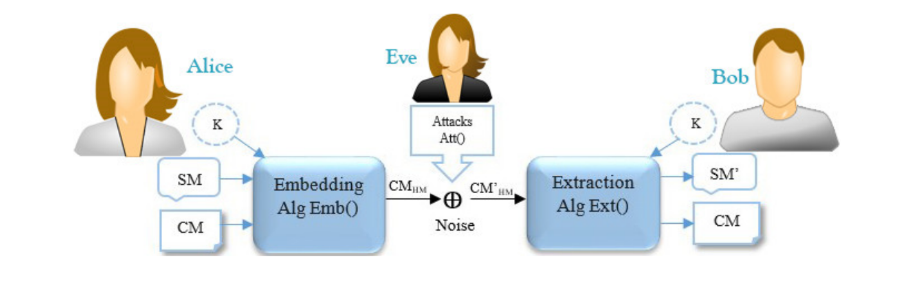
\includegraphics[scale=0.45]{modern_text_hiding.png}
    \end{figure}
    
    The proposed image intuitively explains the logic of the schema.
    Alice who whishes to send a Secret Message(SM) to Bob, will produce a Cover
    Message(CM), \emph{i.e.} an innocent message which will work as a carrier.
    She will then embedd the SM into the CM using a steganographic algorithm
    and, optionnally\footnote{This is the domain of cryptography}, securing it
    with a key(K).
    In the end she will pass the message to Eve, who will analyse it before
    giving it to Bob.
    Eve, an active warden, will use steganalysis tools in order to break the
    cover taylored by Alice and will possibly distort the message in order to
    make it unreadable to Bob.
    Once the message arrives to Bob, he will apply the inverse steganographic
    algorithm in order to read the message.
    Since the message could be courrupted Bob will have to perform some error
    correction in order to make the message readable again(whenever this is
    possible).
    To summarize the principal charachteristics of the message sent by Alice
    are:
    \begin{itemize}
        \item \emph{invisibility}: the message should not be noted by Eve
        \item \emph{capacity}: the CM must be large enough to embedd all the SM
        \item \emph{distortion roboustness}: the SM should resist the noise
            produced by Eve in the channel
    \end{itemize}

    \subsubsection{Steganography in text}
    Now let us abandon the prison world to move to the digital domain.
    We now want to propose intuitively some algorithm which could be exploited
    to cover hidden messages into text.
    The field of hidden-text encoding owes its growth to two main factors: the
    introduction of the Unicode Standard and the growth in popularity of social
    media and messenger applications.
    The number of "invisible" characters introduced by the Unicode
    standardization can be exploited by steganographic algorithms just as
    invisible ink was exploited in handwritten steganography.
    Combining this result with the fact that the modern society produces every
    year more data than ever before in human history, the possibilities and the
    threats brought by steganography in the digital world are basically
    limitless.

    \begin{figure}[h]
        \centering
        \caption{Text Hiding techniques}
        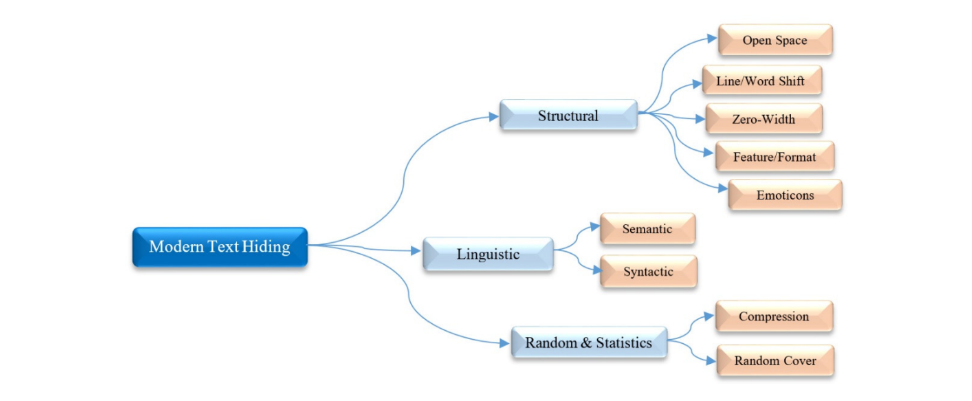
\includegraphics[scale=0.45]{text_hiding.png}
    \end{figure}

    As you can see the field is vast even here and unfortunately we will only
    treat the most interesting points of the numerous ramifications.

    \paragraph{Structural}
    This set of techniques consist in altering the structure of the document
    rather than actively modifying the file. The case of \emph{open space} is
    significant: the spaces are substituted by other invisible Unicode
    character.
    This technique is easily noticeable(even by the human eye) and not so much
    rubust.
    Similar is the \emph{zero width} techniques which exploits the zero width
    characters present in the Unicode standard.
    Even more visible are the format, color and alignement alterations of
    \emph{Format}.
    Much more interesting is the case of \emph{Emoticons} which has found secure
    ground in the last period and which consist of assigning to each emojy a
    code(letter or word).

    \paragraph{Linguistic}
    Much more stable are the algorithms which exploits linguistic
    characteristics in order to hide the presence of hidden bits.
    In the \emph{Semantic} case the message is hidden inside abbreviations or
    achronyms.
    This method provides much more reliability and lower embedding capability
    than the previous one.
    Much worse and visible is the \emph{Syntactic} approach which consists in
    changing symbols with others to represent some code.

    \paragraph{Random and Statistic}
    These method start only from the SM and try to generate a CM.
    They are usually much more time and resources consuming.
    The \emph{Compression} method consists in compressing the text of the SM
    using well known compression algorithms such as \emph{Huffman Coding}.
    The so compressed text is then reordered to mimic the user-typed format or
    at least a plausible one.
    Not much more efficient is the \emph{Random Cover} approach where an
    algorithm(\emph{AH4s}) is used to generate a long(and usually meaninglsess)
    text from the specified SM.
    The latter method is indeed very visible and also computationally expensive.

    \subsubsection{steganalysis}

    \paragraph{visual steganalysis}
    This is a human powered technique which simply consists in reading the texts
    searching for anomalies in the syntax, impagination and type of characters
    used.
    This type of analysis can only be performed by trained users and in most of
    the scenarios simply detects the presence of hidden messagges without
    retreiving it.
    A common type of attack which could be performed by the user consciously(not
    necessarily) is manually changing the structure of the message.
    This may lead to the loss or irretrievability of the SM.

    \paragraph{Statistical steganalysis}
    We have already treated this in the previous section, but now we will focus
    our attention on the particular case of text steganography.
    Since we don't want to treat the topic from a too mathematical perspective,
    we will try not to enter into the mathematical technicalities.
    The basic principle beneath is the assumption that it is possible to
    describe the message with a probability function.
    Recalling some basic principles of probability, if
    $ x_1, x_2, x_3 \dots x_n $ are independent, then
    $ p(x_1, x_2, x_3, ... x_n) = p(x_1) p(x_2) \dots p(x_n)$. 
    Instead when they are not then
    $ p(x_1, x_2, x_3, ... x_n) = p(x_1) p(x_2 | x_1) p(x_3 | x_1, x_2) \dots
    p(x_n | x_1, x_2, \dots, x_{n-1})$.
    Starting by the assumption that written text follows a logic schema and thus
    that words are interdependently related, then by computing the probability
    function of the text and comparing it to the one of the
    \emph{stego-message}(assumed to be perturbed by steganography) we can detect
    the presence of steganography in the text. 
    This tells us that in theory is possible to detect whether a sequence of
    characters follows a specific pattern or not, and it is in theory also
    possible to retrieve the message from such prediction.
    In \cite{fast-steg-method} the experiment presented shows that it is
    possible to use a neural network to recognize patterns into text messages
    which are proper of \emph{stego-messages}.

    \subsection{TCP/IP}
    \subsubsection{Introduction}
    Before treating such topic we must briefly discuss the behaviour of the
    TCP/IP (\textbf{Internet protocol suit}) communications.
    
    \paragraph{IP (Internet Protocol)} is at the basis of internet
    communication. The protocol exploits the principle of encapsulation, sending
    packets composed by a \emph{header} which contains information such as the
    \textbf{destination address} and \textbf{source address} and a
    \emph{payload} which represents the actual data to be transmitted.
    Since physical channels usually have a limited \emph{MTU}\footnote{Maximum
    Transmission Unit}, then the data is usually fragmented in smaller chunks,
    wrapped into an header and only then transmitted.
    
    \paragraph{TCP (Transmission Control protocol)} is a protocol used for
    reliable (little information loss), ordered, error-checked data transmission
    between a machine hosting the data (\textbf{Server}) and another requiring
    such data (\textbf{Client}). It is performed previous a three-way handshake
    which estabilishes a connection between server and client, thus preparing a
    reliable communication channel.

    \paragraph{UDP (User Datagram Protocol)}, contrary to TCP, is less reliable
    but faster.
    It broadcasts the data in an unordered and uncontrolled way to the receiver. 
    There is no need to estabilishing a connection in order to implement such
    protocol.

    \begin{figure}[h]
        \centering
        \caption{Structure of TCP packet}
        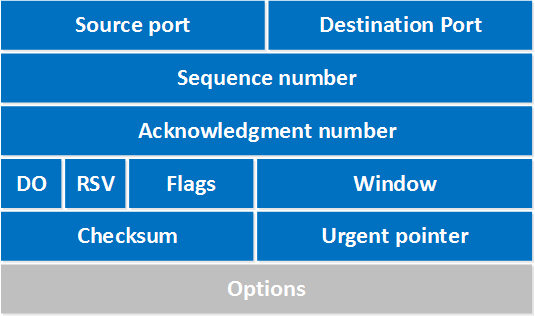
\includegraphics[scale=0.5]{tcp_header.png}
    \end{figure}

    \begin{figure}[h]
        \centering
        \caption{Structure of UDP packet}
        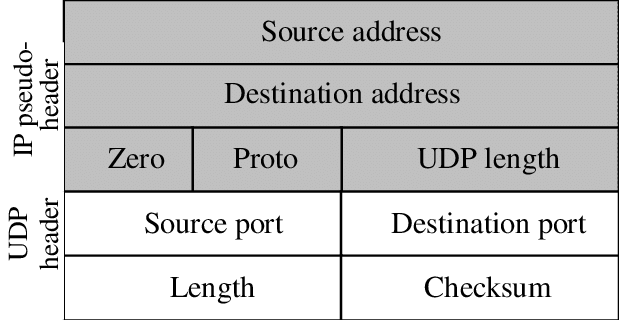
\includegraphics[scale=0.3]{udp_header.png}
    \end{figure}

    \subsubsection{Exploits and protection tools}

    As you could notice from the previous figures, the first part of the header
    is the same. This is because it is part of the IP protocol itself.
    In the second part of each header we find different types of metadata which
    are specific for each protocol. Generally the metadat contained in the
    header is redundant for the transmission of the message itself and this 
    redundancy may become a target for a \emph{stego-algorithm}\footnote{an
    algorithm used for steganography} which starting from a \emph{cover-network
    packet sequence}\footnote{a sequence of packets which will be transmitted
    over the network acting as a cover for the hidden messace} and a
    \emph{covert message}, can generate a sequence of packets(each one embedding
    a portion of the covered message) which will be sent over the network.

    This procedure is not a \emph{risk-free} approach for the attacker who
    wishes to send the \emph{cover-network packet sequence}, since it is
    possible that the data will be currupted during transmission or there could
    be losses using non-reliable transport protocols(UDP).
    Other criticalities of such method stay in the fact that the sequence of
    packets will most likely traverse multiple nodes in the network before
    reaching the target, and the message may be detected by these nodes.

    The defense against Steganography in TCP/IP communication consists in 
    series of standards which are implemented by the devices on the internet and
    that we will illustrate through some examples.


    \paragraph{Tof(Type of service)} bits are a field in the TCP header which
    are nowdays rarely used. This could open doors to a steganographic attack if
    modern operating systems did not set them to zero by default.
    A warden monitoring the channel could immediately signal an error.

    \paragraph{IP ID} is a field in the Internet Protocol which is used to
    assist the receiver in reassemblying the fragmented packets.
    This field consist of randomly unique numbers representing a packet.
    It is possible to insert other types of information in this field by simply
    conform to the uniqueness constraint.
    Since in many cases the numbers used for the IP ID are not random, by
    knowing the charachteristics of the sender it is possible to detect an
    infiltration.

    \paragraph{IP Fragment Offset} is an offset which is present in the IP
    header which helps the receiver to reconstruct the sequence of bits from the
    fragmented sequence.
    Modulating the size of the fragments changes the offset field in the header
    and thus a message could be sent.
    The protection against this method is simply checking the size of the
    packets relative to the MTU and so even in this case a warden can easily
    detect an error.

    \paragraph{TCP sequence number} is a field in the TCP header which stores
    the randomly chosen position(for security reasons) of the first byte to be
    transmitted through the channel. The steganographic method consists in
    replacing this field with the data to be sent.
    Being random it is more difficult to spot a breach in the channel.
    In this case the usage of a \emph{SVM}\footnote{Support Vector Machine}, a
    machine learning tool able to identify patterns inside the data transmitted
    could come into hand.
    However an error could be detected even simply by checking the presence of
    repetitions in the stream(not admitted by design). 

    \paragraph{Timestamp modulation} is another technique of steganography which
    operate by modifing the \emph{LSB} of the
    timestamp of a TCP packet in order to represent a '1'.
    The covert message is thus embedded into the data stream.
    Since the TCP Timestamp support is not universal, machines not supporting
    such feature may detect the hidden message.


    \subsubsection{Detection of TCP/IP steganography}

    Each operating system exhibits well defined characteristics in generated
    TCP/IP fields. These can be used to identify any anomalies that may indicate 
    the use of steganography. For this purpose, a suite of tests which may be
    applied to \emph{network traces}\footnote{function that performs network
    analysis on a geometric network} are defined and they are used to identify
    whether the results are consistent with the operating systems believed to be
    installed on the source host.
    Diffreent methods of covert channel detection are used, employing IP ID 
    characteristics, TCP ISN characteristics and explicit steganography
    detection.

    \paragraph{IP ID characteristics} are the features identifying the IP
    address, a unique address that identifies a device on the internet or local
    network. They are employed by the following methods.
    \emph{Sequential Global IP ID} implies the usage of a global counter for the
    IP ID. 
    To detect this strategy one has to look if connections to different hosts
    have sequentially increasing IP IDs.
    \emph{Sequential Per-host IP ID} is characterized by the usage of a per-host
    counter for packets. If it apperas to be fragmented, the warden can test
    whether connections to different hosts use apparently unrelated IP IDs;
    however connections to the same host have a sequentially increasing IP ID.
    \emph{IP ID MSB Toggle} represents the case where the operating system
    system toggles the most significant bit of the IP ID every rekey interval,
    so that the warden can examine the MSB to check if it matches this pattern.
    \emph{IP ID Permutation} strategy presence can be discarded by the warden if
    there are duplicates, since within a rekey interval the IP ID is
    non-repeating.

    \paragraph{Explicit steganography detection} can be employed by several
    methods.
    \emph{Nushu Criptography} is a strategy applied by Nushu, which encrypts
    data before including it in the ISN field, resulting in a distribution which
    differs form the one that is normally generated by Linux; therefore, it can
    be detected. 
    \emph{TCP Timestamp} strategy involves the execution of a randomness test.
    In particular, if a low bandwidth TCP connection is being used to leak
    information, this test can be applied to the LSBs of the timestamps in the
    TCP packets. If an excessive presence of randomness is detected in the LSBs,
    it can be deduced that a steganographic covert channel is in use.
    There are also other features which may indicate the usage of steganography:
    \emph{unsual flags}, \emph{excessive fragmentation}, use of \emph{IP
    options}, \emph{unexpected TCP options} and \emph{excessive re-ordering}.

    \pagebreak

\end{document}